% 11 pages
This chapter will lay foundations for medical imaging for clinical diagnostics and the basic methodology used throughout this thesis to tackle advanced imaging diagnostics.

\section{Clinical Background: Volumetric Medical Imaging} %4 pages

% Ideas:
% zhang2024challenges (foundation models in deep learning)
% https://3dqlab.stanford.edu/what-is-3d-imaging-2/

    \subsection{Diagnostic Disciplines and Tasks} %1 pages
        With the development of the CT scanner by Godfrey Hounsfield in the late 1960s, taking volumetric images of the body became possible and was used and researched with increasing effort in the following decades \citep{alexander2010emi, rubin2014computed}. Volumetric \ac{CT} images can be used to diagnose and plan the treatment of several diseases and conditions such as stroke, vascular diseases, cancer (see \chapref{chap:deepstaple}), trauma, acute abdominal pain and diffuse lung disease \citep{rubin2014computed}. With volumetric \ac{CT} images an exact evaluation of  three-dimensional measures such as tumor growth and estimation
        of doubling times % (271) TODO orig source of doubling times
        and analyzing the three-dimensional shape became possible \citep{rubin2014computed}. Similarly other volumetric quantities could be measured such as the volume of the
        left cardiac ventricle,  % TODO orig source (343)
        cerebral spinal fluid, % TODO orig source (344)
        liver and spleen % TODO orig source (345)
        and tumoral neoplasia. % TODO orig source (346)
        CT in its current state has excellent spatial resolution and distinguishing tumors given that tumors and the surrounding tissue provide enough contrast \citep{abramson2023surgeons}.
        But the three primary objectives of radiologists, namely the detection, resolution and characterization of abnormalities \citep{abramson2023surgeons} might not be satisfied when tissue does not provide enough contrast on X-ray beams.
        % utting-edge CTtechniques, including the use of more sensitive photon counting de-tectors3 and dual energy data acquisition,4,5 will increase CT spatial resolution and contrast while minimizing noise, but this is unlikely toovercome the multitude of MR sequences tailored to images varioustissues throughout the body.  \citep{abramson2023surgeons}

        \ac{MRI}, which is available commercially since the early 1980s, has superior contrast over CT regarding soft-tissue \citep{abramson2023surgeons, kabasawa2022mr}. \ac{MRI} sequences can be specifically tailored towards the application regarding. This requires a trade-off beetween sufficient \ac{SNR}, voxel volume and acquisition time under the influence of the examined object\footnote{A more in-depth explanation can be found in \ref{chap:acquisitionfocus}} \citep{macovski1996noise}. E.g. T2 sequences suppressing fat are excellent for tumor detection, where tumors are displayed brighter than the dark, suppressed fat, but spatial resolution is rather coarse with 5mm thick slicing gaps \citep{abramson2023surgeons}.
        \ac{MRI} can be used in various applications such to assess brain and heart function (see \chapref{chap:deepstaple} and \chapref{chap:acquisitionfocus}), abdominal organs such as liver and pancreas (see \chapref{chap:dgtta}) and knee cartilage \citep{mazurowski2019deep}.

        % Within this con-text, the need to reformat, reconstruct,and render CT images into alternativedisplays was driven by a desire to pro-vide all physicians with an understand-ing of the anatomic nuances that CT provided in a manner that might been countered in the surgical suite. Al-though computers and computation arefundamental to CT, the applications ofcomputer graphics, vision, and quan-titation methods were not sufficientlymature to make their use routine un-til the latter days of the 20th century. \citep{rubin2014computed}


        % s. One quickly meet challenges associated to memoryand compute consumption when using CNNs with higher-dimensional image data, challenges thatresearchers are trying various approaches to deal with (treating 3D as stacks of 2Ds, patch- orsegment-based training and inference, downscaling, etc). It is clear that the ideas behind state-of-the-art two-dimensional CNNs can be lifted to three dimensions, but also that adding a thirdspatial dimension results in additional constraints. \citep{lundervold2019overview}

        % DL specific
        % \citep{litjens2017survey}
        % \citep{piccialli2021survey}

        % TODO Why is US not explained in this thesis?

        % How did volumetrict Medical Imaging evolve
        % CT and MRI are often done paired follow ups? This is why these are in focus.
        % CT (and PET) and MRI are important imaging domains.

    \subsection{Imaging Domains and Scanner Properties} %1.5 pages

        \begin{figure}
            \begin{minipage}{\textwidth}
                \centering
                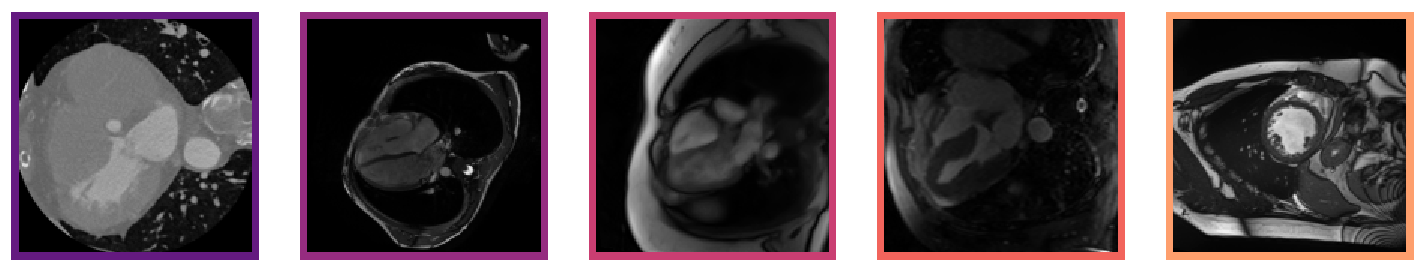
\includegraphics[width=.89\textwidth]{sections/02_background/figures/contrast_imgs.pdf}
                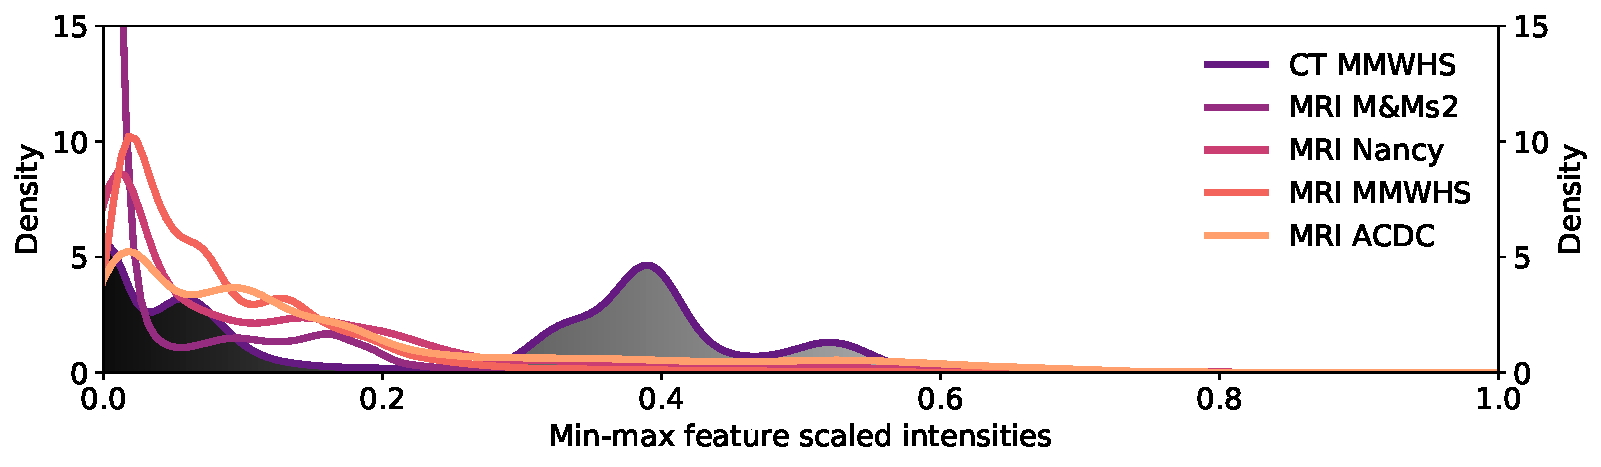
\includegraphics[width=\textwidth]{sections/02_background/figures/contrast_histograms.pdf}
                \caption{Top: One \ac{CT} and several \ac{MRI} images of cardiac studies \citep{xx,xx,xx,xx}. Bottom: Histogram of the image intensities each scaled to min-max feature scales. The \ac{CT} histogram is shaded with the corresponding image grayscale intensities. Appearance of \ac{CT} and \ac{MRI} images differ substantially but also \ac{MRI} images have a large variation in appearance due to different scanners and acquisition protocols.}
                \label{fig:domain_contrast}
            \end{minipage}
        \end{figure}

        \figref{fig:domain_contrast}

        \citep{withers2021x}
        % What are the special benefits and downsides of CT, MRI, technically speaking.

        % example images
        % Value ranges (histogram) https://pmc.ncbi.nlm.nih.gov/articles/PMC9011180/pdf/nihms-1794910.pdf
        % Image normalization by scanner (HU vs. MRI)
        % MRI magic triangle T1 weighted / T2 weighted scans
        % slicing MRI vs CT
        % image recovery: MRI k-Space transform, CT Radon transform
        % Acquisition timing
        % Scanner costs



    \subsection{Generalization: Challenges and Possibilities} %1.5 pages
    % Number of manufacturers, number of MRI sequences
        % Studies that show problems with generalization for CT / MRI
        % Studies that show approaches to overcome scanner domain gaps
        % What makes Generalization hard?

        % What can be done to achieve generalization in each of the steps?

\section{Methodological Background: Deep Learning} %7 pages
    % TODO: This needs to be a lot shorter now
    % https://books.google.de/books?hl=de&lr=&id=qOF4AgAAQBAJ&oi=fnd&pg=PP1&ots=vNTiX5Lu_U&sig=UEC7rljJ7dVsAbh_XQeMmCrNqcU#v=onepage&q&f=false
    The principal mechanisms of learning were studied in the last century by investigating conditioned learning, where an outcome is associated to a stimulus by a learning organism e.g. a dog that awaits food after hearing the sound of a bell \citep{pavlov1928conditioned, pavlov2010conditioned, banich2011generalization}. Later, fear responses were especially studied and two sub-mechanisms of conditioned learning --- generalization and specialization --- were discovered \citep{banich2011generalization}.
    In fear learning, initially an instance-based generalization occurs that maps a novel fear to an environment \citep{banich2011generalization}. Later, this generalization is specialized and mapped to specific environmental stimuli leading to discrimination \citep{banich2011generalization}.
    It was discovered, that generalization can occur intra-modal and cross-modal for the example of the food awaiting dog either receiving visual or auditory stimuli \citep{pavlov1928conditioned} and that gradients of generalization exist \citep{guttman1956discriminability}.
    The concept of gerneralization and spezialization can be tracked down to individual parts of the brain, where the initial generalized learning is associated to the amygdala whereas the specialization occurs in the prefrontal cortex and the hippocampus \citep{banich2011generalization}.

    On the cell level, learning and building memory is assumed to work as the change of neuron connection-strength through synaptic plasticity \citep{do1949organization,martin2000synaptic}. Apart from synaptic information exchange it was also figured out that information exchange occurs volumetrically between glia cells and neurons with extracellular vesicles in the nervous system \citep{schiera2019communcation}.

    \subsection{Basic Principles} % 1 pages
        % https://cs.stanford.edu/people/eroberts/courses/soco/projects/neural-networks/History/history1.html

        Inspired by the research findings in biological learning processes, \citeauthor{mcculloch1943logical} decribed several parts of network structures mimicking neural systems \citep{mcculloch1943logical}.
        Over a decade later \citeauthor{rosenblatt1957perceptron} developed the concept of a \emph{perceptron} as a learning element for electronic or electromechanical systems to recognize patterns \citep{rosenblatt1957perceptron}.
        First real classification experiments were conducted by \citeauthor{widrow1960adaptive} using small neural networks \citep{widrow1960adaptive}.
        % TODO: were those exp based on value tables? vs. backprop?
        More than two decades later the \emph{Backpropagation} mechanism was developed, that is nowadays used in current deep learning approaches to systematically configure the weights and biases of neural networks \citep{rumelhart1986learning}.

        % With increasing computational power and availability of large data through the internet machine learning techniques experienced increased interest \citep{xx}.

        \paragraph{Backpropagation} The basic principle of deep learning is the backpropagation mechanism.

        \begin{align}
            \diffp{E}{{y_j}} &= y_j - d_j \\
            \diffp{E}{{x_j}} &= \diffp{E}{{y_j}} \cdot \diffp{{y_j}}{{x_j}}
        \end{align}

        % Now that we know how deep learning works in general, we can have a look at individual building blocks models / data concepts / supervision tasks

    \subsection{Data Representation and Model Architectures} % 2 pages

        \subsubsection{Convolutional Neural Networks}
            % cnns, unets
            % cnn Kernels
        \subsubsection{Graph Neural Networks}
            % feature aggregation
            % rota groups, equivariance,

    \subsection{Training and Optimization Strategies} % 3 pages
        % curriculum learning, dice loss
        % metrics

    \subsection{Generalization: Recent Discussion and Approaches} % 1 pages
        % What are the current approaches in deep learning? How is the idea of AGI related to our gerneralization approach? What can be problems of AGI and why do we analyse generalization in a limited scope such as medical image analysis?
        % generalization methods